\documentclass[a4paper,12pt]{jarticle}
\newcommand{\setcounters}[1] {
  \setcounter{equation}{#1}
  \setcounter{figure}{#1}
  \setcounter{table}{#1}
}

\newcommand{\unit}[1] {
  \hspace{1mm}\mathrm{[#1]}
}

\newcommand{\degc} {
  \hspace{1mm}\mathrm{[}{}^\circ\mathrm{C]}
}

\newcommand{\refig}[1]{Fig.\ref{fig::#1}}
\newcommand{\refeq}[1]{式(\ref{eq::#1})}
\newcommand{\reftab}[1]{Tab.\ref{tab::#1}}

\newcommand{\fig}[5] {
  \begin{figure}[#1]
    \begin{center}
      \includegraphics[width=#2\hsize]{#3}
    \end{center}
    \caption{#4}
    \label{fig::#5}
  \end{figure}
}

\makeatletter
\def\eq{\@ifstar\@eq\@@eq}
\def\@eq#1{\begin{equation*}#1\end{equation*}}
\def\@@eq#1#2{\begin{equation}#2\label{eq::#1}\end{equation}}
\makeatother

\newcommand{\diff}[2] {
  \frac{\mathrm{d}#1}{\mathrm{d}#2}
}

\newcommand{\pdiff}[2] {
  \frac{\partial #1}{\partial #2}
}


\newcommand{\ddt}[2][1] {
  \ifnum #1 < 2
    \frac{\mathrm{d}#2}{\mathrm{d}t}
  \else
    \frac{\mathrm{d}^#1#2}{\mathrm{d}t^#1}
  \fi
}

\newcommand{\e}[1] {
  \mathrm{e}^{#1}
}

\newcommand{\lparen}{(}
\catcode `( = \active
\newcommand{(}{\ifmmode\left\lparen\else\lparen\fi}

\newcommand{\rparen}{)}
\catcode `) = \active
\newcommand{)}{\ifmmode\right\rparen\else\rparen\fi}

\newcommand{\bmat}[1] {
  \begin{bmatrix} #1 \end{bmatrix}
}

% -- Package ---------------------------------------------------
\usepackage{fancyhdr}
\usepackage{here}
\usepackage{listings}
\usepackage[dvipdfmx]{graphicx}
\usepackage{amsmath,amssymb,epsfig}
\usepackage{eucal}
\usepackage{bm}
\usepackage{ascmac}
\usepackage{pifont}
\usepackage{multirow}
\usepackage{enumerate}
\usepackage{cases}
\usepackage{type1cm}
\usepackage{cancel}
\usepackage{url}
\usepackage{cite}
\usepackage{color}
%\usepackage[dvipdfmx]{color}
\usepackage{caption}
\usepackage[caption=false]{subfig}
\captionsetup[figure]{labelsep=space}
\usepackage[ruled,vlined]{algorithm2e}
\usepackage{setspace}
\usepackage{comment}
\DeclareRelationFont{JY1}{mc}{it}{}{OT1}{cmr}{it}{}
\DeclareRelationFont{JT1}{mc}{it}{}{OT1}{cmr}{it}{}
\DeclareFontShape{JY1}{mc}{m}{it}{<5> <6> <7> <8> <9> <10> sgen*min
    <10.95><12><14.4><17.28><20.74><24.88> min10
    <-> min10}{}
\DeclareFontShape{JT1}{mc}{m}{it}{<5> <6> <7> <8> <9> <10> sgen*tmin
    <10.95><12><14.4><17.28><20.74><24.88> tmin10
    <-> tmin10}{}
\DeclareRelationFont{JY1}{mc}{sl}{}{OT1}{cmr}{sl}{}
\DeclareRelationFont{JT1}{mc}{sl}{}{OT1}{cmr}{sl}{}
\DeclareFontShape{JY1}{mc}{m}{sl}{<5> <6> <7> <8> <9> <10> sgen*min
    <10.95><12><14.4><17.28><20.74><24.88> min10
    <-> min10}{}
\DeclareFontShape{JT1}{mc}{m}{sl}{<5> <6> <7> <8> <9> <10> sgen*tmin
    <10.95><12><14.4><17.28><20.74><24.88> tmin10
    <-> tmin10}{}
\DeclareRelationFont{JY1}{mc}{sc}{}{OT1}{cmr}{sc}{}
\DeclareRelationFont{JT1}{mc}{sc}{}{OT1}{cmr}{sc}{}
\DeclareFontShape{JY1}{mc}{m}{sc}{<5> <6> <7> <8> <9> <10> sgen*min
    <10.95><12><14.4><17.28><20.74><24.88> min10
    <-> min10}{}
\DeclareFontShape{JT1}{mc}{m}{sc}{<5> <6> <7> <8> <9> <10> sgen*tmin
    <10.95><12><14.4><17.28><20.74><24.88> tmin10
    <-> tmin10}{}
\DeclareRelationFont{JY1}{gt}{it}{}{OT1}{cmbx}{it}{}
\DeclareRelationFont{JT1}{gt}{it}{}{OT1}{cmbx}{it}{}
\DeclareFontShape{JY1}{mc}{bx}{it}{<5> <6> <7> <8> <9> <10> sgen*goth
    <10.95><12><14.4><17.28><20.74><24.88> goth10
    <-> goth10}{}
\DeclareFontShape{JT1}{mc}{bx}{it}{<5> <6> <7> <8> <9> <10> sgen*tgoth
    <10.95><12><14.4><17.28><20.74><24.88> tgoth10
    <-> tgoth10}{}
\DeclareRelationFont{JY1}{gt}{sl}{}{OT1}{cmbx}{sl}{}
\DeclareRelationFont{JT1}{gt}{sl}{}{OT1}{cmbx}{sl}{}
\DeclareFontShape{JY1}{mc}{bx}{sl}{<5> <6> <7> <8> <9> <10> sgen*goth
    <10.95><12><14.4><17.28><20.74><24.88> goth10
    <-> goth10}{}
\DeclareFontShape{JT1}{mc}{bx}{sl}{<5> <6> <7> <8> <9> <10> sgen*tgoth
    <10.95><12><14.4><17.28><20.74><24.88> tgoth10
    <-> tgoth10}{}
\DeclareRelationFont{JY1}{gt}{sc}{}{OT1}{cmbx}{sc}{}
\DeclareRelationFont{JT1}{gt}{sc}{}{OT1}{cmbx}{sc}{}
\DeclareFontShape{JY1}{mc}{bx}{sc}{<5> <6> <7> <8> <9> <10> sgen*goth
    <10.95><12><14.4><17.28><20.74><24.88> goth10
    <-> goth10}{}
\DeclareFontShape{JT1}{mc}{bx}{sc}{<5> <6> <7> <8> <9> <10> sgen*tgoth
    <10.95><12><14.4><17.28><20.74><24.88> tgoth10
    <-> tgoth10}{}
\DeclareRelationFont{JY1}{gt}{it}{}{OT1}{cmr}{it}{}
\DeclareRelationFont{JT1}{gt}{it}{}{OT1}{cmr}{it}{}
\DeclareFontShape{JY1}{gt}{m}{it}{<5> <6> <7> <8> <9> <10> sgen*goth
    <10.95><12><14.4><17.28><20.74><24.88> goth10
    <-> goth10}{}
\DeclareFontShape{JT1}{gt}{m}{it}{<5> <6> <7> <8> <9> <10> sgen*tgoth
    <10.95><12><14.4><17.28><20.74><24.88> tgoth10
    <-> tgoth10}{}
\endinput
%%%% end of jdummy.def



% -- Margin Config ---------------------------------------------
\addtolength{\topmargin}{-\headheight}
\addtolength{\topmargin}{-\headsep}
\addtolength{\textheight}{-60truemm}

% -- Layout Config ---------------------------------------------
\setlength{\hoffset}{0cm}
\setlength{\oddsidemargin}{-3mm}
\setlength{\evensidemargin}{-3cm}
\setlength{\marginparsep}{0cm}
\setlength{\marginparwidth}{0cm}
\setlength{\textheight}{24.7cm}
\setlength{\textwidth}{17cm}
\setlength{\topmargin}{-45pt}



% -- Renewcommand ----------------------------------------------
\renewcommand{\theequation}{\arabic{section}.\arabic{equation}}
\renewcommand{\thefigure}{\arabic{figure}}
\renewcommand{\thetable}{\thesection.\arabic{table}}
\renewcommand{\lstlistingname}{ソースコード}
\renewcommand{\headrulewidth}{0mm} % fancy
\renewcommand{\labelenumi}{(\arabic{enumi})}
\renewcommand{\baselinestretch}{1.3}
\renewcommand{\floatpagefraction}{1}
\renewcommand{\topfraction}{1}
\renewcommand{\bottomfraction}{1}
\renewcommand{\textfraction}{0}
\renewcommand\thefootnote{\arabic{footnote})}
\renewcommand{\figurename}{Fig.}
\renewcommand{\tablename}{Tab.}



% -- Config for fancy package ----------------------------------
\pagestyle{plain}
\rhead{\thepage}
\lhead{}
\cfoot{}


% -- Config for counter ----------------------------------------
\setcounter{section}{0}
\setcounter{subsection}{0}
\setcounter{subsubsection}{0}
\setcounter{equation}{0}

% 式番号を式(章番号.番号)に
\makeatletter
\renewcommand{\theequation}{\arabic{section}.\arabic{equation}}
\@addtoreset{equation}{section}
\makeatother


% -- Config for package listings -------------------------------
\lstset{
  basicstyle={\ttfamily \small},
  breaklines=true,
  frame=trBL,
  numbers=left,
  numberstyle={\ttfamily \small},
}



% 表紙
\title{修士論文\\
産業用ロボットの力覚センサを組み込んだ\\柔軟指の開発\\
% {\large No title}
}
\author{\vspace{90mm}\\
指導教員:\ 黒木 \hspace{0mm} 秀一 教授\\
九州工業大学大学院\ \hspace{0mm} 工学府\\
工学専攻\ \hspace{0mm} 知能制御工学コース \\
\vspace{0mm}\\
学籍番号:\ 193D2007\\
提出者氏名:\ 川崎 \hspace{0mm} 雄太朗\\\vspace{5mm}\\ }
\date{令和3年\ 2月\ 12日}

\begin{document}

%表紙
\titlepage
\maketitle
\thispagestyle{empty}
\newpage
\addtocounter{page}{-1}

% 目次
\thispagestyle{empty}
\begin{abstract}
現在,日本の人口減少における工場の労働者不足を補うためにロボットによる省人化が求められている.その中で産業用ロボットは様々な作業に幅広く対応するためにエンドエフェクタの交換を行う.把持,搬送,組付け作業を行うエンドエフェクタはグリッパと呼ばれる.グリッパの交換には作業ごとのグリッパ選定や把持計画の再実施を行わなければならず作業効率の低下につながる.この問題を解決するため汎用的に作業できるユニバーサルグリッパの開発が行われている.昨今ユニバーサルグリッパには汎用的な把持性能だけでなく組付け作業に対応可能な力覚機能の需要が増えている.力覚機能を有するロボット用の指研究の多くは産業用途対応する耐久性を持たない.そこで本研究では耐久性と把持性能を両立する柔軟指に力覚機能を付加させ性能を検証した.ラティス構造を有する2種類の柔軟指を作成し汎用的な把持のできる内骨格型グリッパを用いた.
\end{abstract}
\newpage
\thispagestyle{empty}
\addtocounter{page}{-2}
\tableofcontents


%以下それぞれの章
\newpage
%序論
\section{序論}
\label{sec:序論}
産業用ロボットは一般的に把持,搬送,組付けなどの作業をグリッパと呼ばれるエンドエフェクタで行う.グリッパは各作業用に専用設計されていることが多く,作業工程が変わるたびに交換がなされており,最適なグリッパの選定や各グリッパごとに複雑な把持計画を必要とする\cite{nishida}.近年グリッパの交換をせず様々な作業を遂行できる汎用性の高いユニバーサルグリッパの研究がなされている\cite{end}.\par
ユニバーサルグリッパにも様々な種類があり,それらは多関節グリッパ,柔軟グリッパ,内骨格型柔軟グリッパに大別される.多関節グリッパは複数の関節をもつ指を持ちそれらが対象物に倣うことで把持を行う\cite{takansetsu}.\par
多関節グリッパの代表例としてROBOTIQ社のROBOTIQ ADAPTIVE GRIPPER 3-FINGER MODELを\refig{robotiq}に示す.問題点は把持時の接触部を増やすために指の関節を増やすことが求められ機構が複雑になる点が挙げられる.\par
柔軟グリッパは把持部に柔軟膜を有し把持対象物の形状にあわせて変形する特徴がある.対象物に倣い接触面積と摩擦力を増やすことで把持を行う.柔軟グリッパの例としてジャミンググリッパがある\cite{jam}.ジャミンググリッパは柔軟膜の中に空気と粒体を有しジャミング転移現象を利用して固化し把持を行う. \par
内骨格型グリッパは内骨格と言われる固い指の表面に柔軟膜を有している.柔軟指部分が把持対象物の形状に倣いつつ内骨格による力拘束が可能である.以上の特徴から対象物の位置決め誤差や計測誤差にロバストであるとともに比較的重い物体の把持が可能である.\par
近年,組付け作業の自動化の需要が高まり汎用的な把持性能にくわえて組付け作業を想定した力覚機能が求められている.\cite{sensor}.\par
過去に開発された力覚機能をもつ柔軟指の例を紹介する.
平井らが開発したホール素子も用いた柔軟指内蔵力覚センサは柔軟指に磁石とホール素子を埋め込み,指先の変形を検知する\cite{hole}.多田らは内部に触覚受容器を持つ人間型柔軟指を開発した.金属棒と二層のシリコンゴムからなる人間の指を模した柔軟指を提案している\cite{ningen}.また,野寺らの研究によりニューラルネットワークをもちいたはめ合い技能の獲得に成功した\cite{hameai}.\par
以上の力覚機能を持つ柔軟指は産業用途における耐久性は考慮されていない.内骨格型グリッパ用に設計された耐久性と柔軟性を両立するラティス構造をもつ柔軟指が提案されている.本研究では内部にラティス構造を有し力覚センサを組み込んだ柔軟指の開発を行う.

\begin{figure}[h]
 \begin{center}
  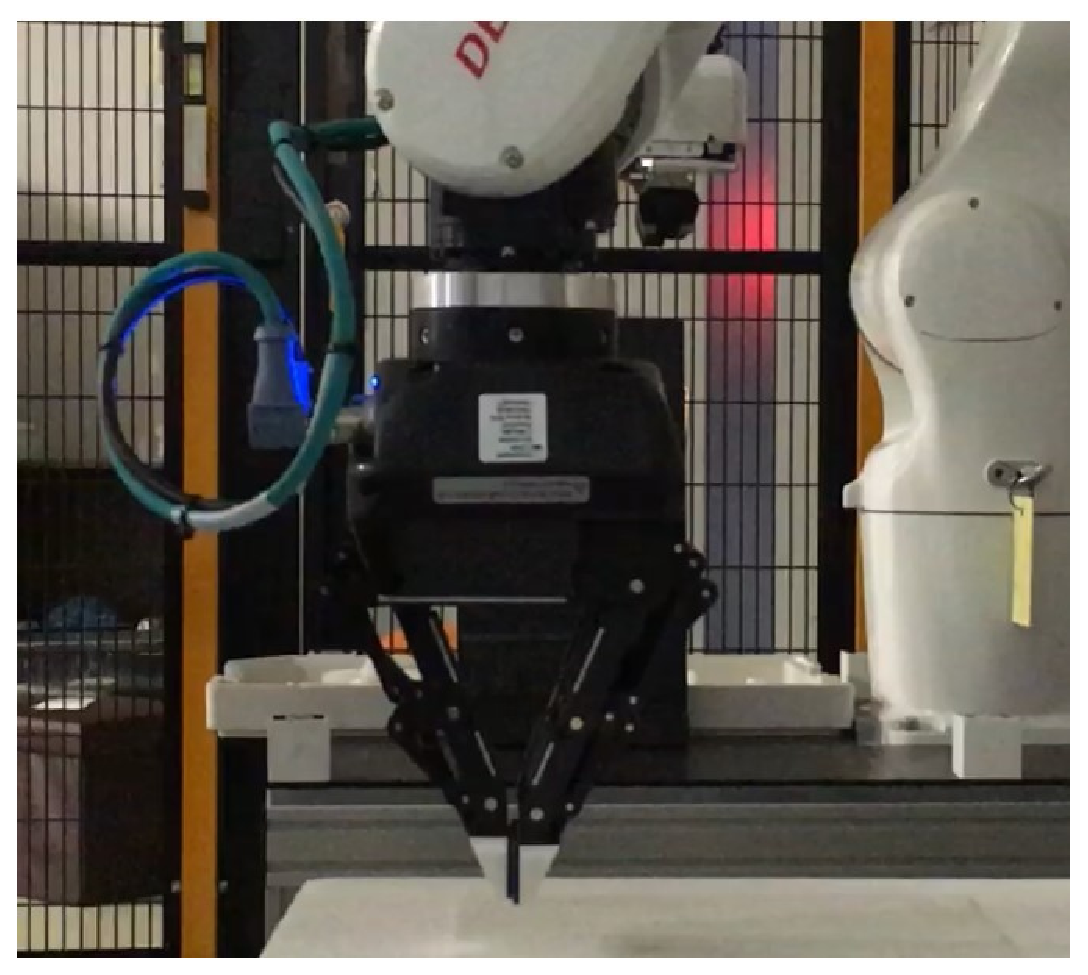
\includegraphics[scale=0.4]{../fig/eps/robotiq.eps}
 \caption{多関節グリッパ}
  \label{fig::robotiq}
 \end{center}
\end{figure}




\newpage
%構造
\section{構造}
\subsection{内骨格型グリッパ}
本研究で用いた内骨格型グリッパを\refig{gripper}に示す.内骨格部分が左右に開閉する並行チャック式である.また中央に押さえ指という把持時に対象物を上方から押さえつけるはたらきをする指がある.本研究ではこの押さえ指は使用していない.

\begin{figure}[h]
\centering
\subfloat[図面]{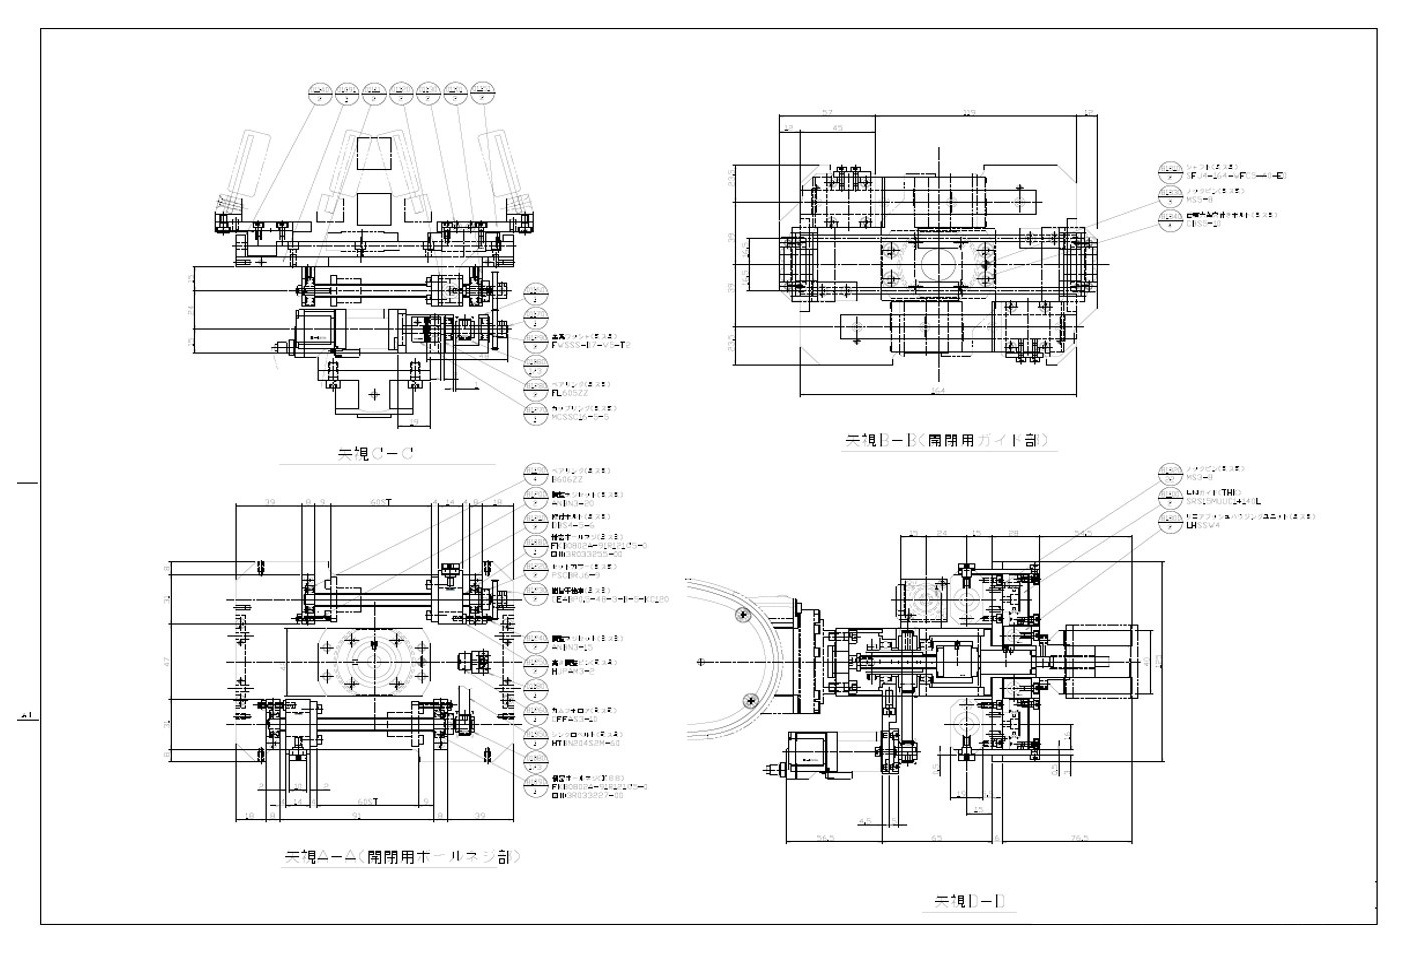
\includegraphics[scale=0.6]{../fig/eps/tercelo_fig.eps}}
\hspace{5mm}
\subfloat[3D図]{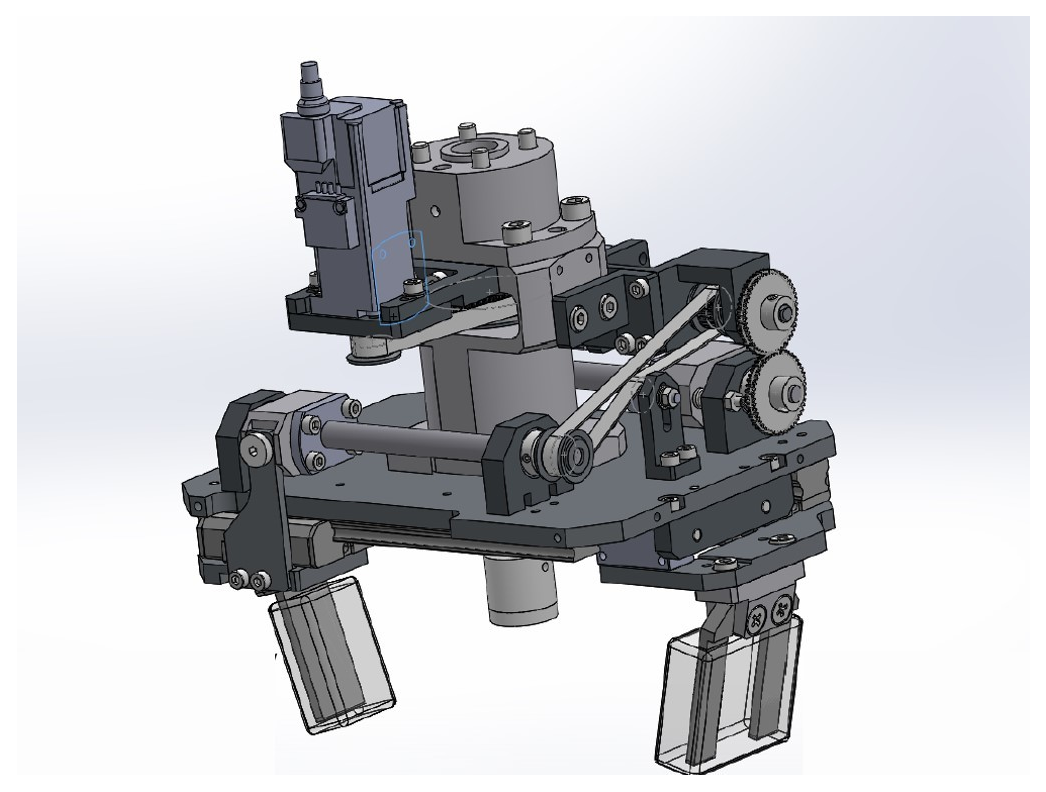
\includegraphics[scale=0.4]{../fig/eps/tercelo.eps}}
\hspace{5mm}
\subfloat[実際のグリッパ]{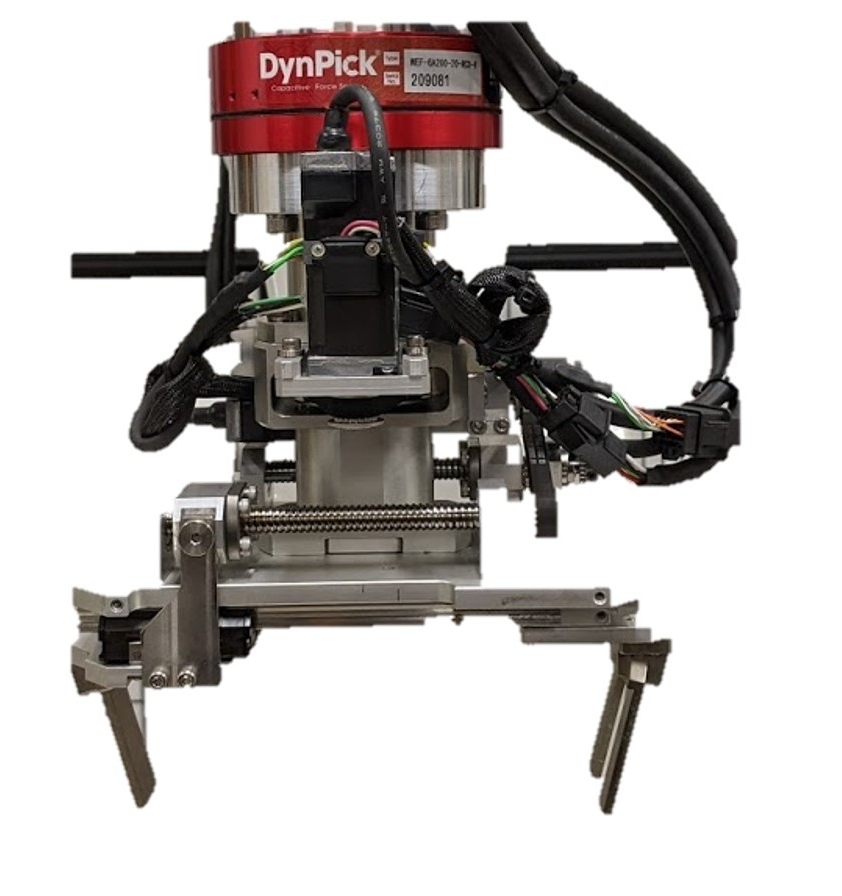
\includegraphics[scale=0.4]{../fig/eps/gripper.eps}}

\caption{内骨格型グリッパ}
\label{fig::gripper}
\end{figure}

\subsection{柔軟指}
本研究では検証に2種類の柔軟指を用いた.いずれも柔軟な把持部にラティス構造を有している.ラティス構造に関しては次の項目で詳しく述べる.3Dプリンタで作成した.使用した3DプリンタはKEYENCE製AGILISTA-3200を用いた.材質はAR-G1H(高硬度シリコン)とした.この材質はショア硬さが35である.主成分はシリコン,アクリルモノマーである.

\subsubsection{通常指}
通常指のCADモデルを\refig{soft_finger_CAD}に実際に作成した指を\refig{soft_finger}に示す.この指は内骨格型グリッパに専用設計された指であるため通常指とした.指上部のスリットに力覚センサを組み込む.

\subsubsection{半球型指}
通常指は対象物に倣うよう設計されているため対象物の荷重が分散しセンシングの感度が疑問視される.ここで高感度で荷重を計測するために半球の凸部とセンサ部が接触するように設計した.この指を半球型指とする.半球型指のCADモデルを\refig{sm_cad},実際に作成した指を\refig{sm}に示す.半球形の把持部の中に通常指と同じパラメータのラティス構造を設けた.

\begin{figure}[h]
\centering
\subfloat[正面]{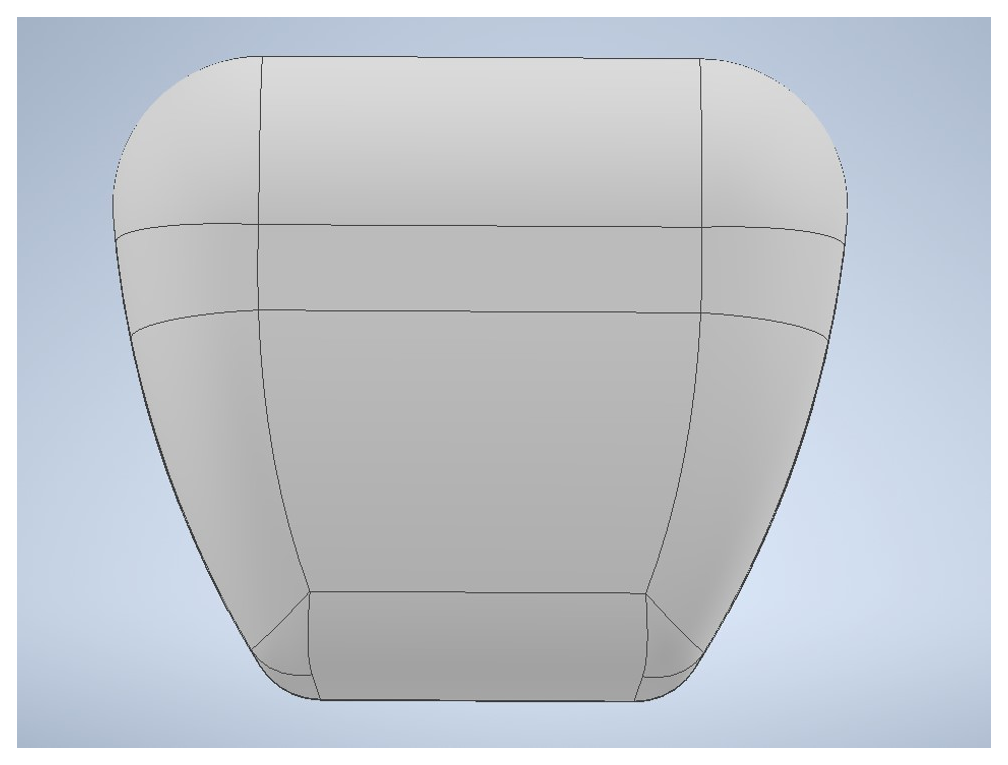
\includegraphics[scale=0.3]{../fig/eps/sf_cad_front.eps}}
\hspace{5mm}
\subfloat[断面図]{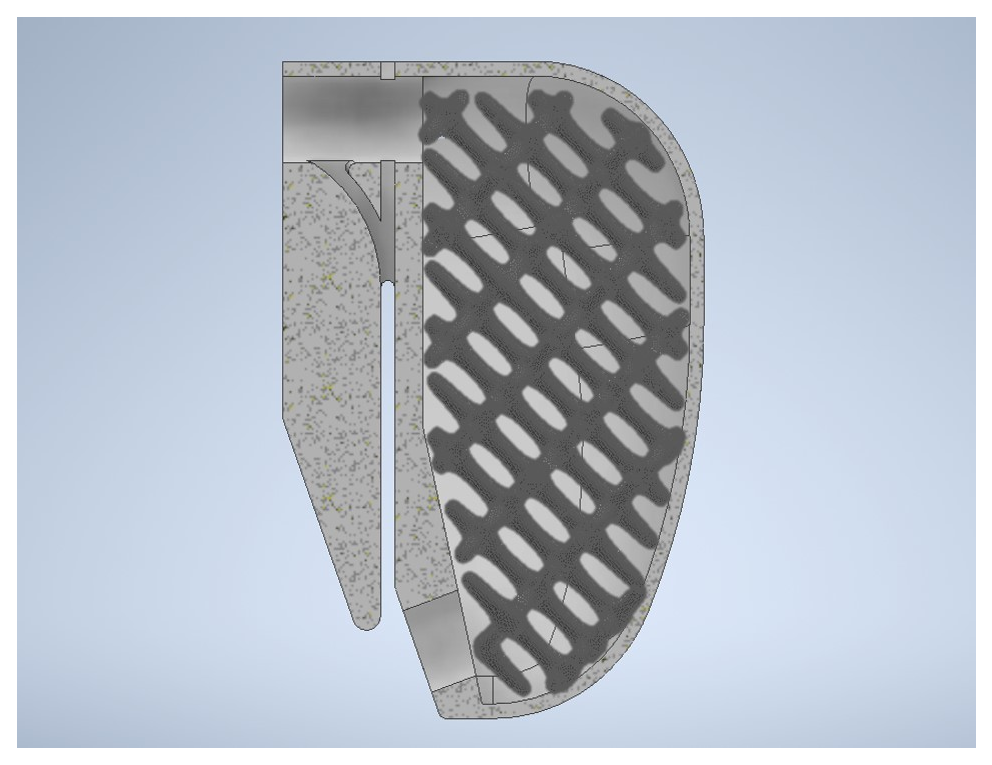
\includegraphics[scale=0.3]{../fig/eps/sf_cad_side.eps}}
\caption{通常柔軟指CADモデル}
\label{fig::soft_finger_CAD}
\end{figure}

\begin{figure}[h]
\centering
\subfloat[正面]{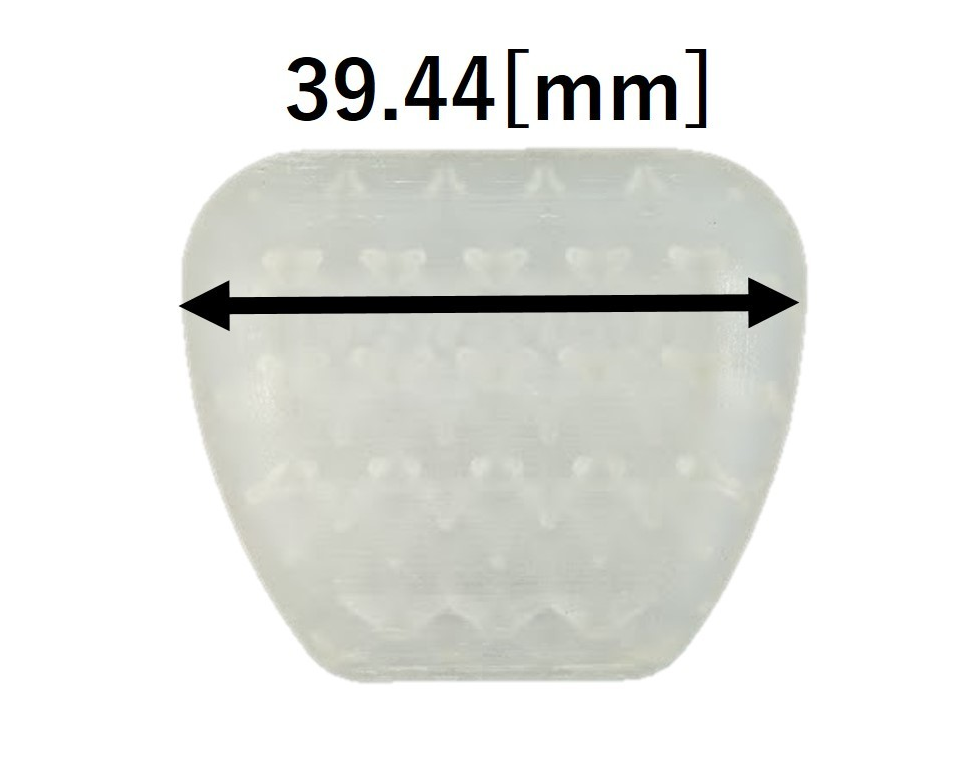
\includegraphics[scale=0.3]{../fig/eps/sf_front.eps}}
\hspace{5mm}
\subfloat[横]{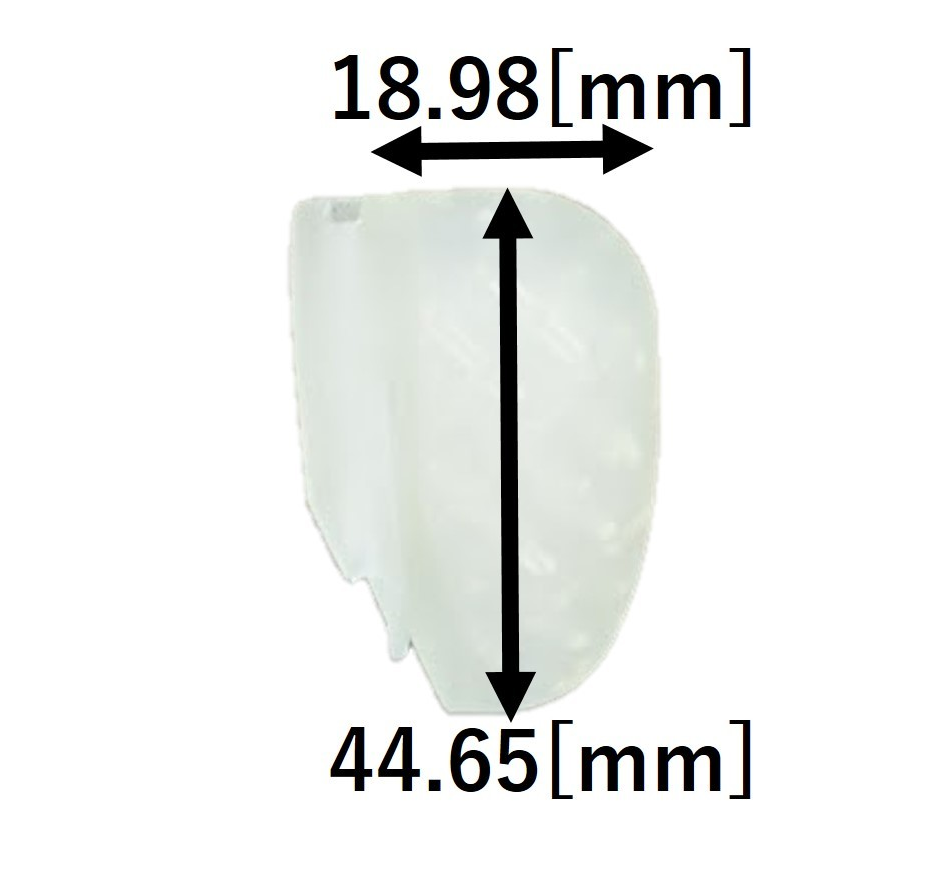
\includegraphics[scale=0.3]{../fig/eps/sf_side.eps}}
\caption{作成した通常柔軟指}
\label{fig::soft_finger}
\end{figure}

\begin{figure}[h]
\centering

\subfloat[正面]{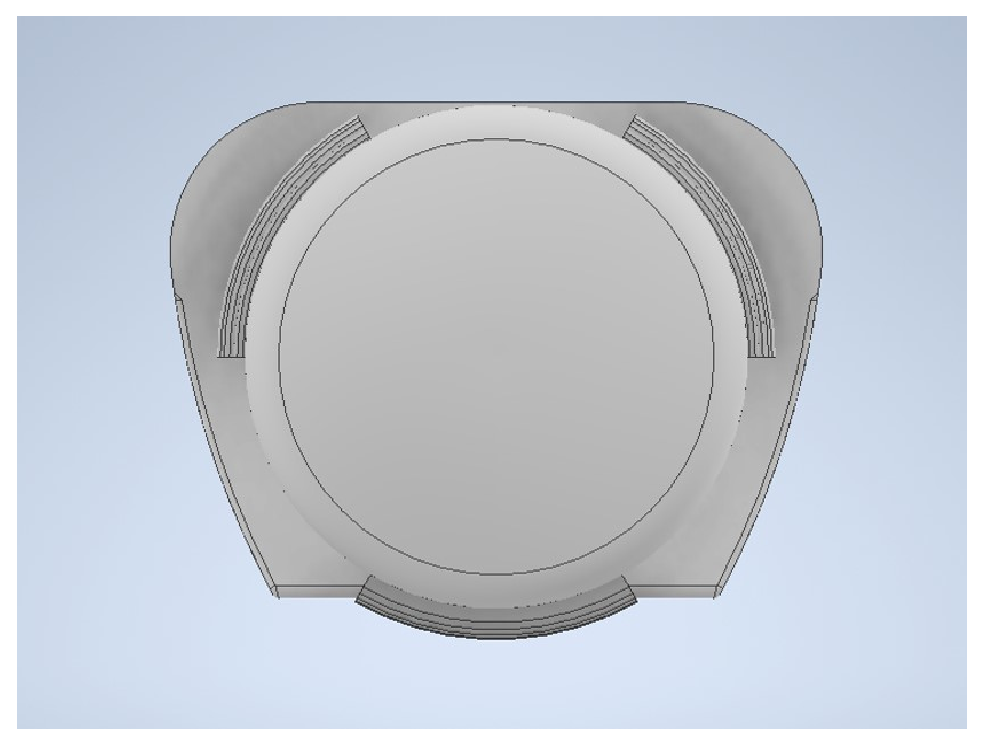
\includegraphics[scale=0.3]{../fig/eps/sm_cad_front.eps}}
\hspace{5mm}
\subfloat[断面図]{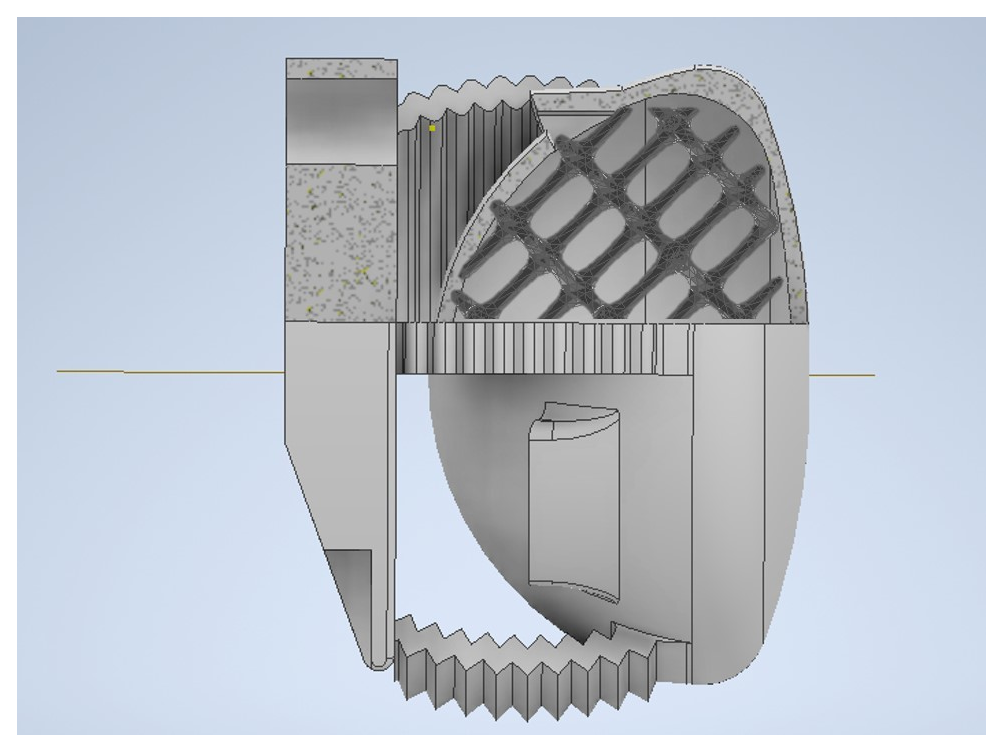
\includegraphics[scale=0.3]{../fig/eps/sm_cad_side.eps}}
\caption{半球型柔軟指CADモデル}
\label{fig::sm_cad}
\end{figure}

\begin{figure}[h]
\centering
\subfloat[正面]{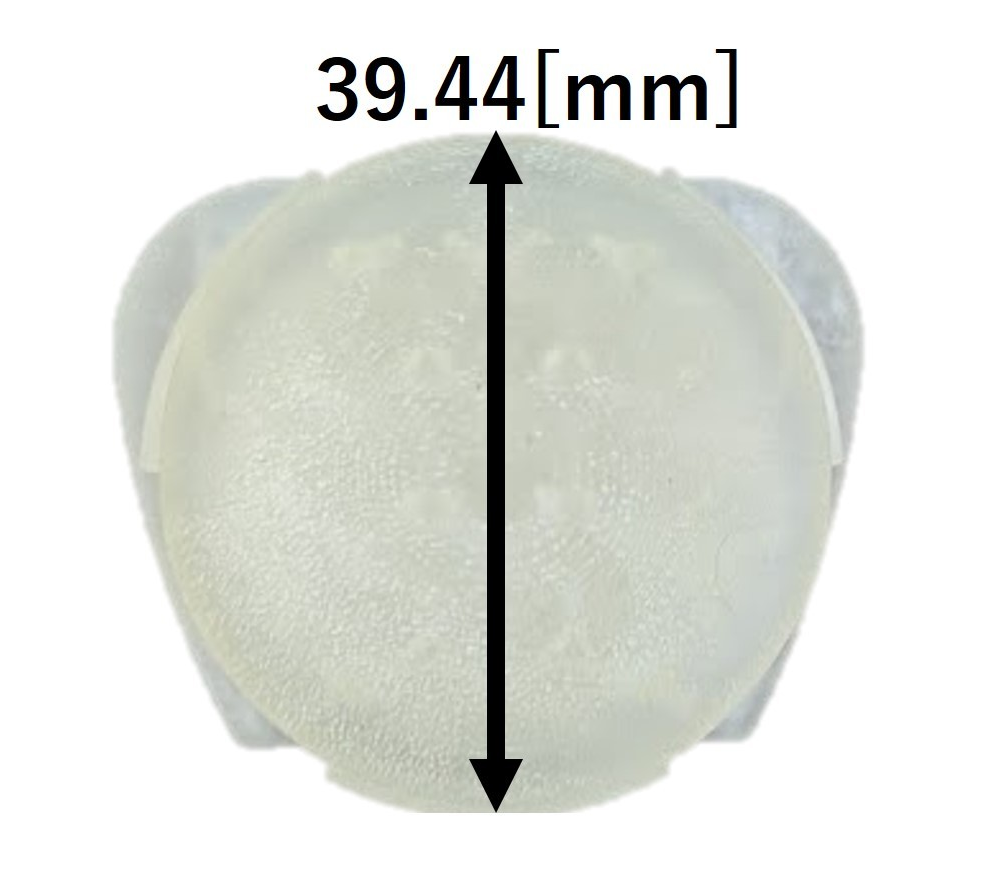
\includegraphics[scale=0.3]{../fig/eps/sm_front.eps}}
\hspace{5mm}
\subfloat[横]{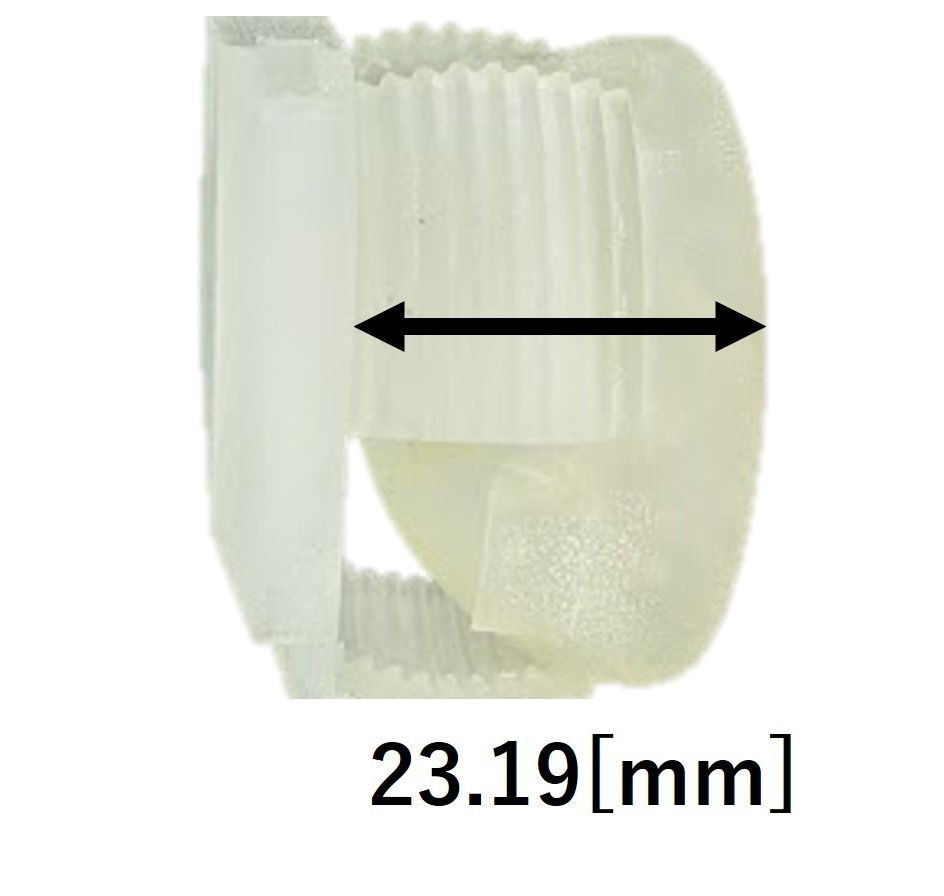
\includegraphics[scale=0.3]{../fig/eps/sm_side.eps}}
\caption{作成した半球型柔軟指}
\label{fig::sm}
\end{figure}

\clearpage

\subsection{ラティス構造}
ラティス構造とは\refig{latice}に示す最小の繰り返し単位が周期的に繰り返される3次元構造で、機械的な強度を損なうことなく軽量化を可能とする\cite{latice}.ラティス構造の特徴として3次元構造の形状や周期のパラメータを変更することができ変形量や内部応答を制御することが可能である.本研究ではAutodesk社製のNetfabbを用いてラティス構造の作成を行いその時のパラメータを\reftab{prm}に示す.


\begin{figure}[h]
\centering
\subfloat[ラティス構造(通常)]{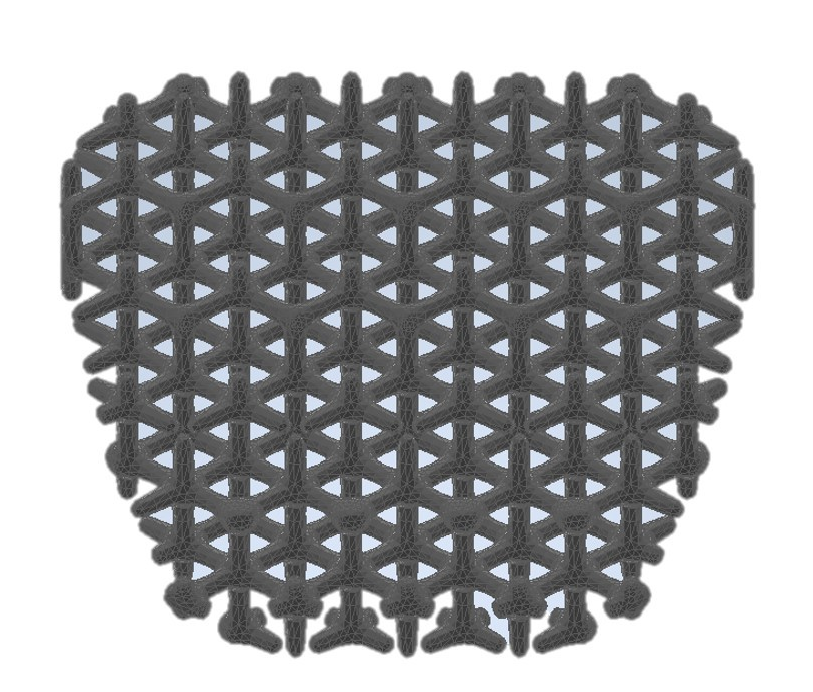
\includegraphics[scale=0.5]{../fig/eps/sf_latice.eps}}
\hspace{5mm}
\subfloat[ラティス構造(半球型)]{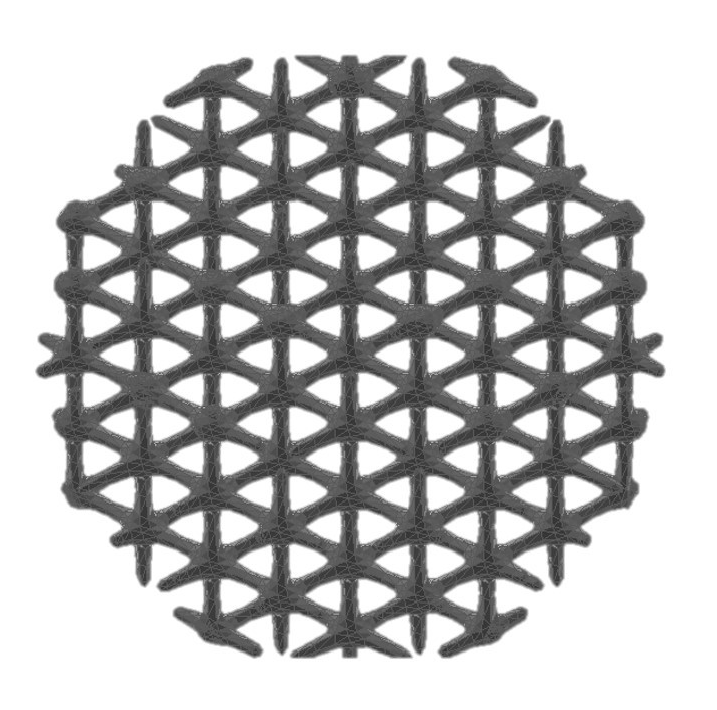
\includegraphics[scale=0.5]{../fig/eps/sm_latice.eps}}
\caption{各指のラティス構造}
\label{fig::latice}
\end{figure}

\begin{table}[htbp]
    \caption{ラティス構造パラメータ} 
  \label{tab::prm}
   %\scalebox{3}[1.5]
  \centering
   \begin{tabular}{|c||c|} \hline
      unit topology & Soft Box  \\ \hline
        Unit size(X,Y,Z) & (8.000mm,8.000mm,8.000mm)  \\ \hline
    Ofset(X,Y,Z) & (0.000mm,0.000mm,0.000mm)  \\ \hline		
    Thickness & (0.671mm)  \\ \hline
    Lattice angle & (0.0deg)  \\ \hline	
    \end{tabular}
\end{table}

\newpage


\subsection{力覚センサ}
イナバゴム社のイナストマーを用いた.\refig{ina}に示す.イナストマーは感圧導電性エラストマー(加圧導電性ゴム)\cite{kanatsu}というゴムを利用した力覚センサである.

\subsubsection{動作原理}
感圧伝導性エラストマーは主にシリコンゴムと導電性粒子(カーボン)から成り立つ.無加圧状態で高い絶縁性を持つが,加圧されるとイナストマーチップ内の導電性粒子が次第に接触しはじめ導電経路が形成され電気抵抗値が低下する.また、減圧して無加圧にするとゴムの弾性による復元力で再度非接触状態に戻る\cite{inabagomu}.

\begin{figure}[h]
\centering
\subfloat[イナストマー]{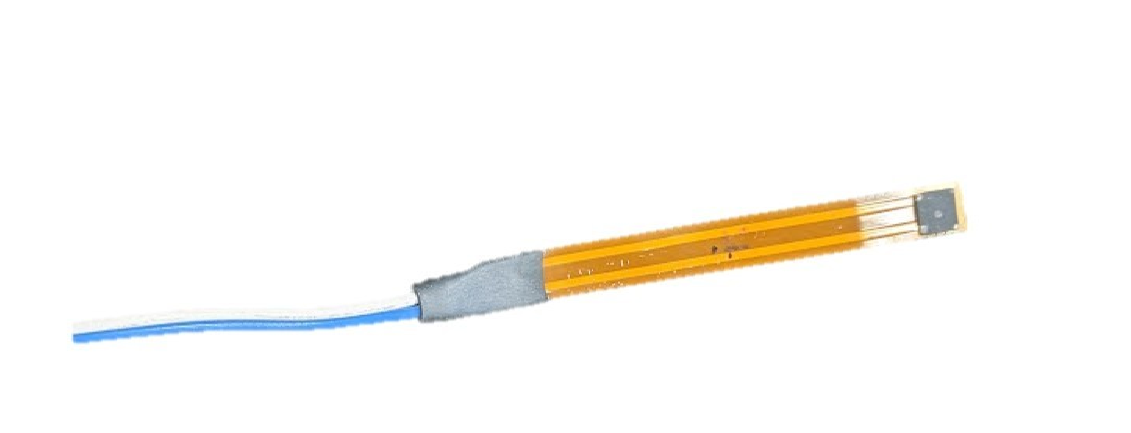
\includegraphics[scale=0.55]{../fig/eps/ina.eps}}
\hspace{5mm}
\subfloat[仕様図]{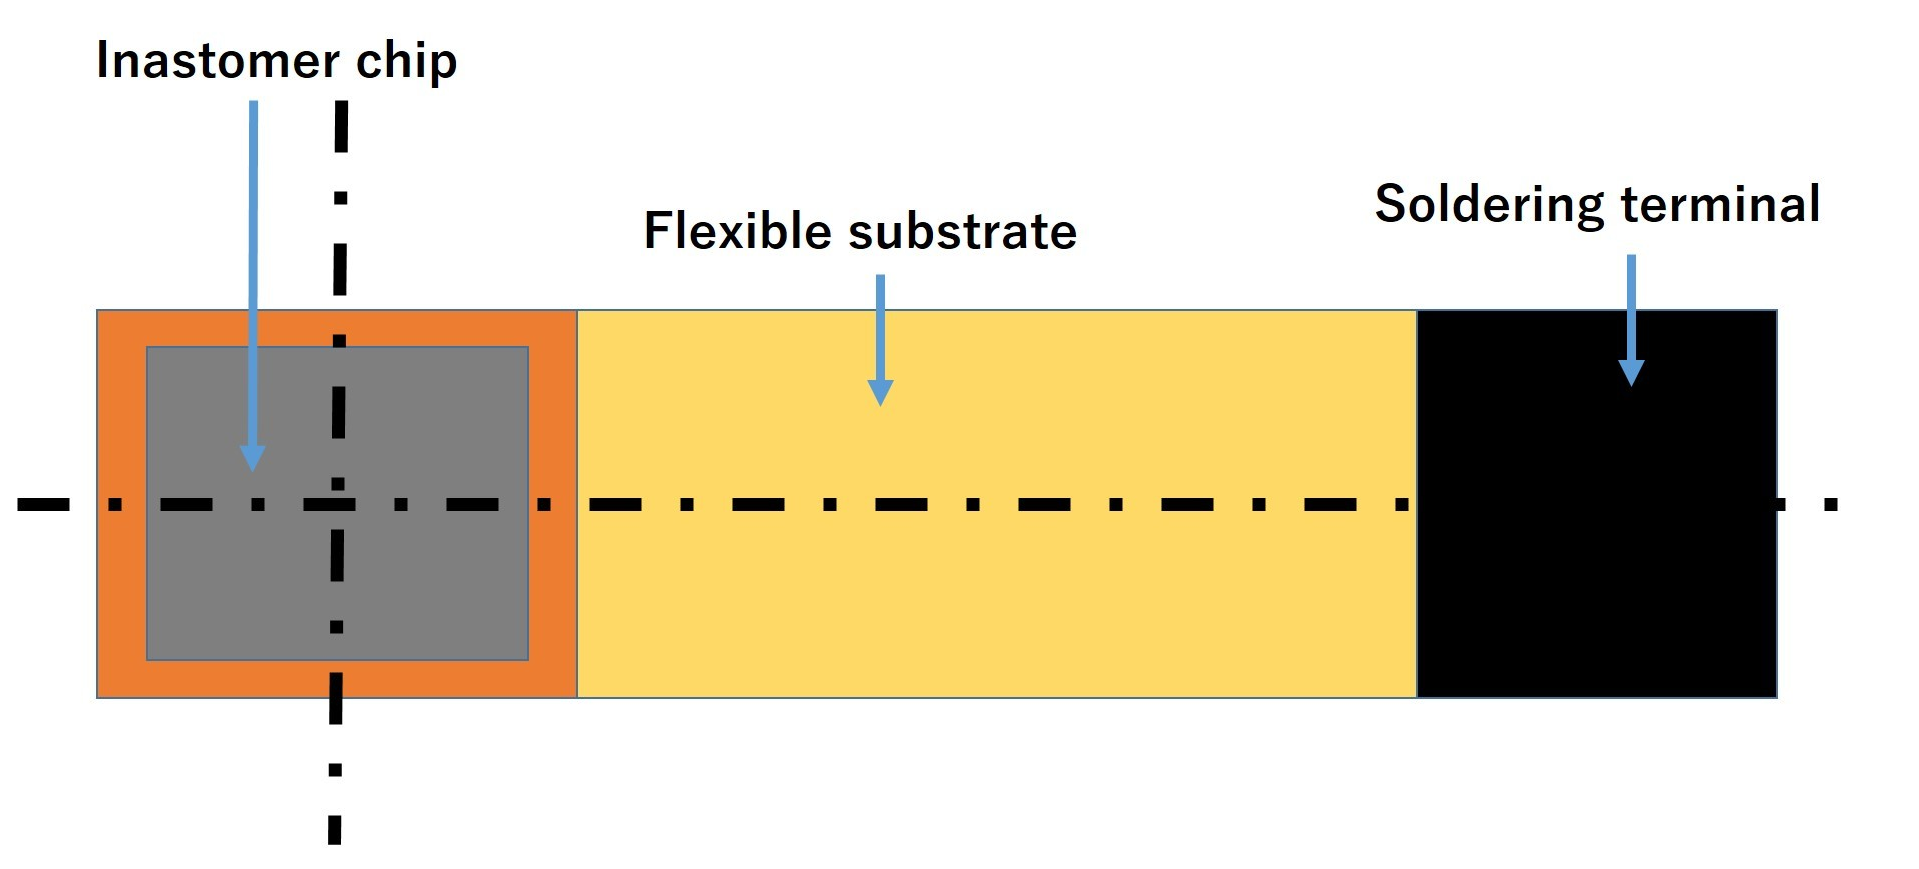
\includegraphics[scale=0.4]{../fig/eps/ina_fig.eps}}
\caption{イナストマー}
\label{fig::ina}
\end{figure}

\newpage




\newpage
%実験
\section{実験}
\subsection{把持実験}
力覚センサを組み込んだ柔軟指で把持対象物を把持したときのセンサの応答を検証した.実験手順は以下の通りである.把持対象物を\refig{objecht}に示す.計測誤差結果を\refig{result0}に示す.

\begin{enumerate}
  \item 力覚センサを組み込んだ柔軟指で対象物を把持する.  
  \item 把持時の力覚センサの電圧値を測定する.
\end{enumerate}

\subsubsection{引張実験}
引張力を検証することで把持対象物に加わる把持力を測定する.以下に実験手順を示す.
実験で使用したフォースゲージを\refig{force_gauge}に示す.

\begin{enumerate}
  \item 力覚センサを組み込んだ柔軟指で対象物を把持する.  
  \item フォースゲージを用いて対象物を鉛直下向きに引っ張った.
  \item 
\end{enumerate}把持対象物が動いたときの引っ張り力を計測した.

\subsection{結果と考察}

\newpage


%\subsubsection{実験結果}
%使用した指は以下の通りである.実験結果を\reftab{result}にまとめる.把持成功は◯,把持失敗は×を表している.把持対象物Eは上部の突起部と下部の外周部での把持が両方成功した時把持成功とみなした.\reftab{result}の横軸は\refig{denso_parts}の割り振った記号と対応し縦軸は以下の指の番号と対応している.

%\begin{enumerate}
  %\item 柔軟物のない指
  %\item 厚さ3mmのゲルを取り付けた指
  
  
%\end{enumerate}

%\begin{table}[htbp]
 %   \caption{把持実験結果}
 
%  \label{tab::result}
   %\scalebox{3}[1.5]
  % \centering
   %\begin{tabular}{|c||c|c|c|c|c|} \hline
      %    &A    &B     &C      &D     &E        %\\ \hline \hline
 %       (1) & ◯ & ◯  & ×  & ◯ & ×  \\ \hline
   %     (2) & ◯ & ◯  & ◯  & ◯ & ◯  \\ \hline
    %    (3) & ◯ & ◯  & ◯  & ◯ & ◯  \\ \hline
	%	(4) & ◯ & ◯  & ◯  & ◯ & ×  \\ \hline
	%	(5) & ◯ & ◯  & ◯  & ◯ & ×  \\ \hline				
	%	(6) & ◯ & ◯  & ◯  & ◯ & ×  \\ \hline
	%	(7) & ◯ & ◯  & ◯  & ◯ & ×  \\ \hline
	%	(8) & × & ×  & ×  & × & ×  \\ \hline		
	%	(9) & × & ×  & ×  & × & ×  \\ \hline		
			
		
    %\end{tabular}
%\end{table}

%\begin{figure}[h]
%\centering
%\subfloat[把持対象物A]{\includegraphics[scale=0.4]{../figure/result_a.eps}}
%\hspace{5mm}
%\subfloat[把持対象物B]{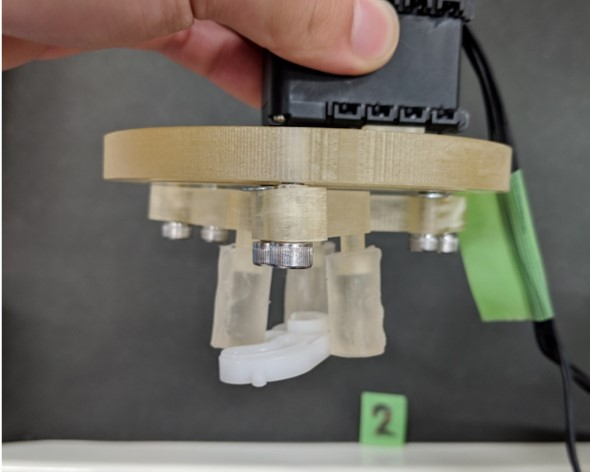
\includegraphics[scale=0.4]{../figure/result_b.eps}}
%\hspace{5mm}
%\subfloat[把持対象物C]{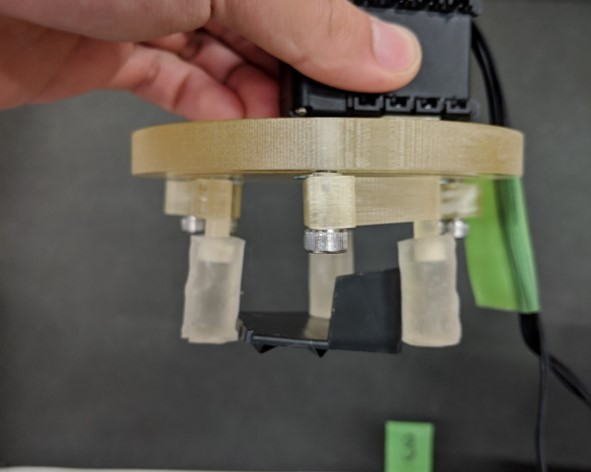
\includegraphics[scale=0.4]{../figure/result_c.eps}}
%\hspace{5mm}
%\subfloat[把持対象物D]{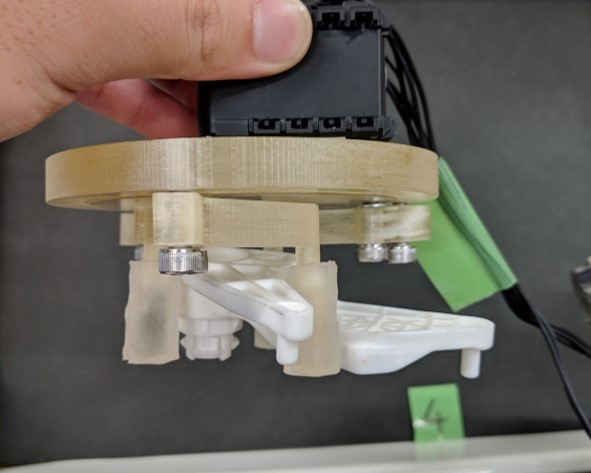
\includegraphics[scale=0.4]{../figure/result_d.eps}}
%\hspace{5mm}
%\subfloat[把持対象物E 上部の突起]{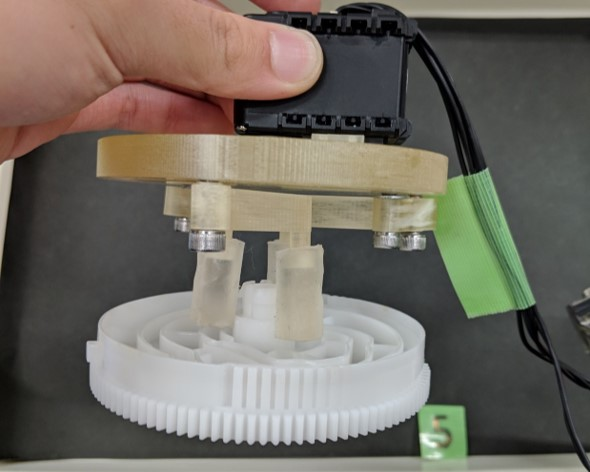
\includegraphics[scale=0.4]{../figure/result_e1.eps}}
%\hspace{5mm}
%\subfloat[把持対象物E 下部の外周部]{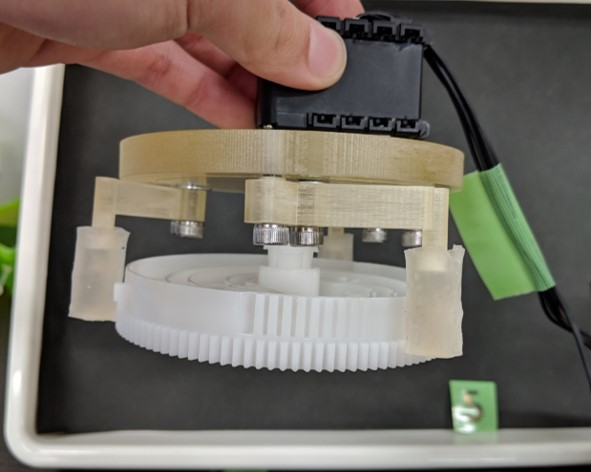
\includegraphics[scale=0.4]{../figure/result_e2.eps}}
%\hspace{5mm}
%\caption{厚さ3mmのゲルの指での把持の様子}
%\label{fig::sisaku}
%\end{figure}



\newpage
%考察
\section{考察}
基礎実験の結果より通常指及び半球型指で把持中には荷重を検出し解放後は荷重を検出しなくなったことからグリッパの把持状態の検出に成功した.\par
荷重実験の結果より通常指はグリッパの把持力が増加に伴う荷重の増加を検出できた.しかし右指と比べて左指は計測した値が小さくなっている.これは左指と対象物の接触位置がセンサ部と離れ十分に力が伝わらなかったからだと考えられる.\\
一方半球型指は球と円筒に関して計測値の左右差はほぼ無くセンサ部に十分力が伝わっている.これは半球型指が押されると半球の凸部に荷重が集中したためであると考察する.ボトルに関して球と円筒に比べて計測値が小さく増減も見られない.これはボトルの把持部であるキャップ部は把持面を上部と下部に分けることができる.上部がキャップのある円筒部の曲面,下部漏斗形の側面が指と接触する.把持の様子を\refig{cap_grasp}に示す.把持時に半球が上下非対称に変形し凸面の位置がずれセンサ部に十分に力がかからなかったと考える.\par
引張実験より\reftab{e3}に通常指と半球型指の対象物ごとの静止摩擦力の差を示す.この表より通常指の方半球型指よりすべての把持対象物で大きく把持時の拘束力が優れていることが
わかる.この理由は通常指のほうが柔軟部が厚く対象物を包む接触面積が大きくなり摩擦力が増加したからであると考えられる.今後の課題として半球型指の把持部をより厚くし拘束力を向上が求められる.

\begin{figure}[htbp]
 \begin{center}u
  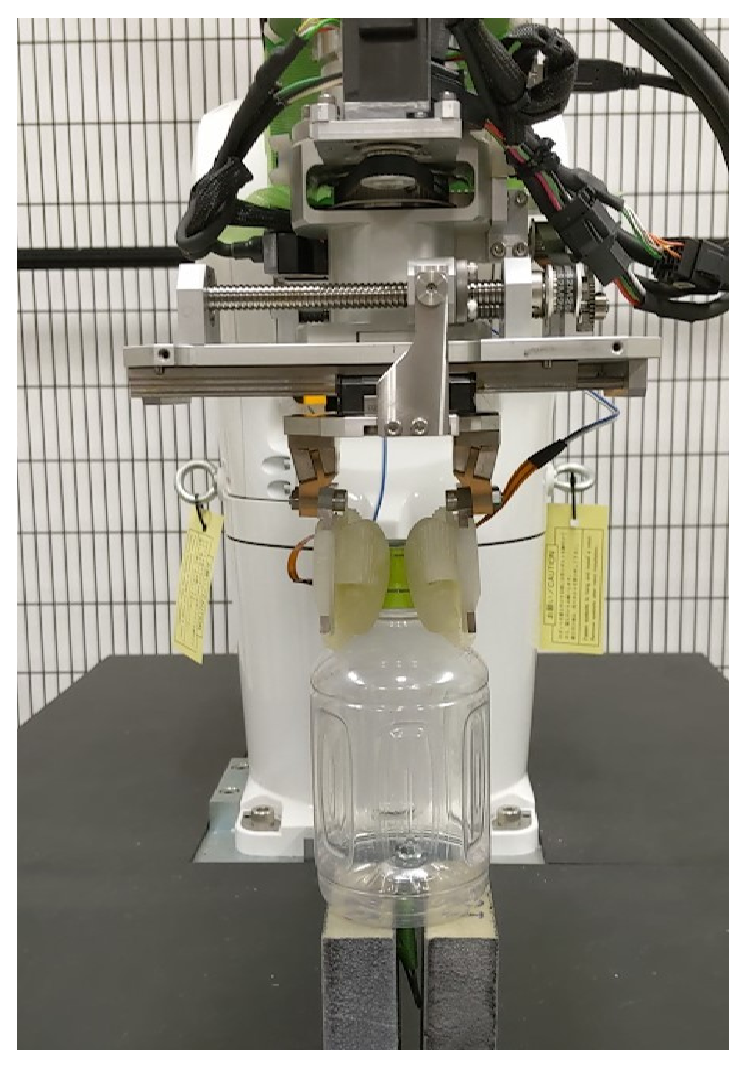
\includegraphics[scale=0.4]{../fig/eps/cap_grasp.eps}
 \caption{半球型指でのボトル把持の様子}
  \label{fig::cap_grasp}
 \end{center}
\end{figure}

\begin{table}[t]
    \caption{静止摩擦力比較}
   \label{tab::e3}
   %\scalebox{3}[1.5]
   \centering
   \begin{tabular}{|c||c|c|c|} \hline
   Force[N]   &Ball     &Cylinder      &Bottle    \\ \hline \hline
        15 & 5.63 & 10.68 & 12.56   \\ \hline
        18  & 4.54 & 6.71  & 13.99    \\ \hline
        21  & 7.44 & 11.76  & 10.77    \\ \hline
		24  & 4.63 & 13.46  & 8.97   \\ \hline
		27  & 7.96 & 10.58  & 13.01   \\ \hline			
		30 & 1.44 & 14.96  & 8.92   \\ \hline
		Average  & 5.27 & 11.36  & 11.37   \\ \hline
		 \end{tabular}
\end{table}


%結論
\section{まとめ}
本研究で内骨格型グリッパの力覚センサを組み込んだ柔軟指の開発を行った.ラティス構造を有した2種類の柔軟指を作成し各実験で性能比較した.基礎実験より両指とも把持状態を検出できることを示した.荷重実験により半球型指の方が荷重を高感度で検出できることを示した.引張実験により通常指のほうが対象物の拘束力に性能に優れていることを示し,半球型指の厚さの再設計を今後の課題とした.
%謝辞
% 謝辞
\section*{謝辞}
本論文作成にあたり御指導下さった九州工業大学大学院工学研究院機械知能工学研究系知能制御工学部門西田特任教授及び黒木教授に深く感謝致します.また、日頃よりご協力頂いた機械知能工学科制御工学教室の教職員の皆様ならびに、同教室西田研究室の皆様に感謝致します.



\begin{thebibliography}{99}
\addcontentsline{toc}{section}{参考文献}

\bibitem{nishida} 西田健,”産業用ロボットのためのソフトグリッパ”,日本ロボット学会誌, Vol.37, pp.42-45, 2019.


\bibitem{end} Tetsuyou Watanabe, Kimitoshi Yamazaki, Yasuyoshi Yokoko-hji, “Survey of robotic manipulation studies intending practi-cal applications in real environments -object recognition, softrobot hand, and challenge program and benchmarking-” , Advanced Robotics , Vol. 31, Iss. 19–20, pp. 1114-1132, 2017.

\bibitem{takansetsu} 多田隈健二郎,”包み込み式グリッパ機構の原理および具体化”,日本ロボット学会誌, Vol.35, p.36, 2017.

\bibitem{jam}J. R. Amend Jr, E. Brown, N. Rodenberg, H. M. Jaeger, H. Lipson: “A Positive Pressure Universal Gripper Based on the Jamming of Granular Material,”IEEE trans. on Robotics, Vol.28, pp.341350, 2012.

\bibitem{sensor} 長久保晶彦,”柔軟な触覚センサ〜実利用に向けて〜”,日本ロボット学会誌, Vol.37, No.5, pp.401-404, 2019.

\bibitem{hole}Damith Suresh Chathuranga,平井慎一,"ホール素子を用いた柔軟指内蔵力覚センサ",http://www.hirailab.com/pub-presents/16/RSJ2016damith.pdf,(2021年2月19日).

\bibitem{ningen} 多田泰徳,細田耕,浅田稔,”内部に触覚受容器を持つ人間型柔軟指”,日本ロボット学会誌, Vol.23, No.4, pp.428-487, 2005.

\bibitem{hameai} 野寺正人,多田泰徳,細田耕,”人間型柔軟指を用いたはめ合い技能の獲得”,日本機械学会ロボティクス・メカトロニクス講演会講演論文集, 巻2006, pp.1A1-B29,2006.

\bibitem{latice}牛島邦晴,Dai-Heng CHEN, Wesley James CANTWELL, 妹尾正隆“3次元ラティス構造のせん断変形特性”日本機械学会論文集77巻781号p.46,2011

\bibitem{kanatsu} 石川正俊,下条誠,"感圧導電性ゴムを用いた圧力センサ",バイオメカニズム学会誌,6巻,3号,p.p.46-51,1982.

\bibitem{inabagomu} イナバゴム株式会社,”イナストマーの原理とメカニズム”,http://www.inaba-rubber.co.jp/products/inastomer/mechanism.html,(2021年2月17日).



\end{thebibliography}

\end{document}
